\chapter{Comparing Stream Processing Frameworks for Cowbird}
In the previous chapter, we have seen that the crucial component of a large-scale streaming infrastructure is a low latency stream processing engine. The big data streaming landscape is constantly growing and many distributed stream processing frameworks are available today. Since we want to extend 
the current Cowbird framework in a way it can support the processing of large amounts of data in real-time, we extensively studied and analyzed some of the stream processing frameworks currently available. We also built a small benchmark framework that helped us understanding which engine is the most suitable for our use case. 

In this chapter, we will discuss the architectural characteristics and main features of the cutting-edge stream processing technologies. We will also describe the benchmark framework we built for evaluating some of the streaming engines described in the following sections. This framework helped us understanding which of the tested streaming engines is the most suitable for our Cowbird architecture.

\section{Overview}
Sensor monitoring, network traffic analysis and security threats detection are some of the applications that generate large amounts of data to be processed in real-time. These stream applications are characterized by an unbounded sequence of events that continuously arrive and need to be processed with a relative low latency. The advent of the Internet-of-Things (IoT) increases the need of real-time monitoring \cite{streamprocessingcomparison}. In fact, Gartner Inc. forecasts that more than 8 billion connected things will be in use worldwide in 2017 and will reach 20.4 billion by 2020 \cite{gartnerarticleonline}. Hence, the amount of data generated cannot always be processed centrally. A distributed architecture is desired in order to process such volume of data.  In these systems, the input data is partitioned and treated in parallel. Thus, high availability and fail recovery are critical in stream processing systems. The stream processing platforms must provide resilience mechanisms against faults, such as delays, data loss, or out of order samples, which are common in a data stream. In low latency applications, the recovery should be quick and efficient, providing processing guarantees \cite{streamprocessingcomparison}. Streaming frameworks usually support one or more of the following processing guarantee semantics:
\begin{itemize}
\item \emph{At-most-once}. Each input sample or message is processed at most one time. In case of failures, the sample/message is not reprocessed.
\item \emph{At-least-once}.  Each input sample or message is processed at lest one time. In case of failures, the sample/message might be reprocessed multiple times and multiple results are delivered.
\item  \emph{Exactly-once}. Each input sample or message is processed once and only once.
\end{itemize}

Stream processing systems have a highly optimized execution engine to provide real-time response for applications with high data-rates. In order to achieve a good processing performance and keeping latency within microseconds streaming platforms minimize communication overheads when data trasmission is required between distributed computations \cite{streamprocessingcomparison}. There are two methods of data processing in streaming processing systems \cite{streamprocessingcomparison}:
\begin{itemize}
\item \emph{Micro-batch processing}. Micro-batch treats the stream as a sequence of smaller data blocks. For small time intervals, the input is grouped into data blocks and delivered to a traditional batch system to be processed.
\item \emph{Stream processing}. The stream processing analyzes and processes massive sequence of unlimited data that are continuously generated. In contrast to micro-batch, it is not limited by any unnatural abstraction.
\end{itemize}

Micro-batch engines have a higher latency in comparison to pure stream processing engines. However, fault tolerance and load balancing are much more efficient in micro-batch processors since, in case of failure, the (micro) batch assigned to the failing node can simply be reappointed to another available machine. Viceversa, in pure streaming engines, fault tolerance is performed for each processed message introducing extra overheads.

The streaming technologies landscape is very rich and there are many streaming engines available. In the following sections, we will briefly discuss the cutting-edge stream processing technologies available right now.

\section{Apache Storm}
One of the most established streaming engines is Apache Storm \cite{apachestormonline}.% It was originally designed at BackType and then open sourced after being acquired by Twitter. 
It has been for years the Twitter's streaming backbone. This system has a pure streaming process engine with a very low latency. However, Storm has also a low throughput and at-least-once processing semantics. In order to add exactly-once semantics to Storm, Twitter created Trident: 
it provides a high-level abstraction on top of Storm that brings exactly-once semantics and \emph{stateful} stream processing (the engine keeps an internal state of the data being processed) to the platform. This is made possible since Trident treats pure streams of data as sequences of micro-batches. Micro-batch incurs to extra latency, even though it increments the throughput. In reaction to these issues, Twitter in 2015 announced Heron \cite{herononline}. Heron was developed internally at Twitter and it provides low latency and high throughput but it has support only for at-least-once and at-most-once processing semantics \cite{streaming@twitter, heron}. 
\section{Apache Samza}
Apache Samza \cite{apachesamzaonline} is an open-source stream processing framework originally developed in conjunction with Kafka at LinkedIn \cite{philosophydistributeddata}. A Samza job consists of a Kafka consumer, an event loop that calls the application code to process incoming messages, and a Kafka producer that sends output messages back to Kafka \cite{philosophydistributeddata}. For each partition of an input topic of a Samza job, a computing unit named StreamTask is allocated. Each task instance consumes messages from just one partition; the task instances can run on the same node or they can be distributed across multiple machines. In Apache Samza, fault tolerance is guaranteed by Kafka. Samza does not implement its own network protocol for transporting messages from one operator to another; all the communications between the computing nodes depend on Kafka \cite{philosophydistributeddata}. Since Apache Samza highly relies on Kafka, it is considered a full-streaming processing engine. However, it also supports batch processing \cite{philosophydistributeddata}. Kafka initially supported only at-least-once semantics, thus Samza has the same degree of processing guarantee. However, Confluent, the company behind Kafka, recently announced the introduction of exactly-once semantics in Apache Kafka in its 0.11 release.

Samza implements durable state within streams of data using a key-value store abstraction. In particular, Samza uses the RocksDB \cite{rocksdbonline} embedded key-value store, which provides low-latency and high-throughput access to data on local disk \cite{philosophydistributeddata}. 

\section{Apache Spark Streaming}
Apache Spark Streaming \cite{apachesparkstreamingonline} extends the Apache Spark framework by introducing the discretized streams (D-Streams) programming model \cite{apachesparkstreaming}. The key idea behind D-Streams is to treat a streaming computation as a series of deterministic batch computations on small time intervals or windows. A discretized stream is just a series of RDDs  grouped together; this series of RDDs contains data arrived within a certain time interval. D-Streams provide both \emph{stateless} operators which act independently on each time interval, and \emph{stateful operators}, such as aggregation over a defined sliding window, which operate on multiple intervals and may produce intermediate RDDs as stream state. Spark Streaming takes care of distributing the state in the cluster, managing it, transparently recovering from failures, and providing fault tolerance.

Fault tolerance is guaranteed in Spark Streaming in the same way it is implemented in Spark; a (micro) batch is simply reassigned to another available node in case of failure. In particular, D-Streams uses an approach called \emph{parallel recovery}. The system periodically checkpoints RDDs state, by asynchronously replicating them to other nodes. When a node fails, the system detects the missing RDD partitions and launches tasks to recover them from the latest available checkpoint. Multiple fine-grained tasks can be launched concurrently in order to compute different RDD partitions on different nodes \cite{apachesparkstreaming}. 

Spark Streaming supports exactly-once sematincs, it has a very high throughput but also a notable latency because of its micro-batching engine \cite{streamprocessingcomparison, yahoobenchmarkingonline, zalandobenchmarkingonline}. 

Spark Streaming also supports full batch processing. Thus, with Apache Spark it is possible to combine stream with batch processing within a single engine.
\section{Apache Flink}
Apache Flink \cite{apacheflinkonline} is an open-source stream processing framework. It is a full stream processing engine and it is based  on its majority on the Google’s Dataflow Model \cite{googledataflow}. Flink supports a full-fledged and efficient batch processor on top of a streaming runtime. Flink executes batch programs as a special case of streaming programs, where the streams are bounded (finite number of elements) \cite{apacheflinkstreamandbatch, apacheflinkstatemanagement}. Both batch and streaming Flink programs eventually compile down to a common representation called the dataflow graph \cite{apacheflinkstreamandbatch, apacheflinkstatemanagement}. The dataflow graph is executed by Flink's runtime engine and it is a directed acyclic graph (DAG) that consists of stateful operators and data streams that flow through these operators: the result stream of an operator is then consumed by another operator in the graph. Since dataflow graphs are executed in a distributed fashion, operators are parallelized into one or more parallel instances called \emph{subtasks} and streams are split into one or more \emph{stream partitions} (one partition per subtask). Stream operators in Flink can be both stateful and stateless. 

Flink supports the notion of \emph{windowing} as in the Google's Dataflow model. Windows split the stream into \emph{buckets} of finite size, over which Flink can apply computations. Flink supports four types of windows when dealing with unbounded data:
\begin{itemize}
\item \emph{Tumbling Windows}. Tumbling windows have a \emph{fixed} size and do not overlap (e.g., five minutes windows, hourly windows or daily windows).
\item \emph{Sliding Windows}. Sliding windows are defined by a window size and slide period (e.g., hourly windows starting every minute). The period may be less than the size, which means the windows may overlap. 
\item \emph{Session Windows}. A session window groups elements by sessions of activity. Session windows do not overlap and do not have a fixed start and end time, in contrast to tumbling windows and sliding windows. Instead a session window closes when it does not receive elements for a certain period of time (i.e a gap of inactivity) occurred. 
%A session window assigner is configured with the session gap which defines how long is the required period of inactivity. When this period expires, the current session closes and subsequent elements are assigned to a new session window.
\item \emph{Global Windows}. Global windows assigns all elements marked with the same key to the same single global window. Since a global window does not have a natural end at which Flink could process the aggregated elements, this windowing mechanism works by specifying a \emph{trigger} that indicates when the elements grouped in the window are ready to be processed. 
\end{itemize}

Windowing mechanisms are time-based. Apache Flink supports three different notions of time in streaming programs:
\begin{itemize}
\item \emph{Processing time}. Processing time refers to the system time of the machine that is executing a certain operation. When a streaming program runs on processing time, all the time-based operations (like time windows) will use the system clock of the compute node that runs the respective operator. Processing time is the simplest notion of time and requires no coordination between streams and machines. It provides the best performance and the lowest latency. 
\item \emph{Event time}. Event time is the time that each individual event occurred on its producing device (e.g., when a data record is produced by a smart city sensor). This time is typically embedded within the data records before they enter Flink and that event timestamp can be extracted from the record. For example, an five minutes event time window will contain all records that carry an event timestamp that falls into that five minutes, regardless of when the records arrive into the system and in what order they arrive. \emph{Event time} gives correct results even on out-of-order events or  late events. In \emph{event time}, the progress of time depends directly on the data, not on any system clocks. \emph{Event time} is implemented through \emph{watermarks}. Watermarks flow as part of the data stream and carry a timestamp \emph{t}. A Watermark(\emph{t}) declares that event time has reached time t in that stream, meaning that there should be no more elements from the stream with a timestamp \emph{t'} $\leq$ \emph{t} (i.e., events with timestamps older or equal to the watermark). \emph{Event time} programs must specify how to generate\emph{Event Time Watermarks}.

\emph{Event time} processing often incurs a certain latency, due to the arrival of late events and out-of-order events. 
\item \emph{Ingestion time}. Ingestion time is the time that events enter Flink. Ingestion time sits conceptually in between event time and processing time. 

Compared to processing time, it is slightly more expensive, but gives more accurate results. Ingestion time uses stable timestamps (assigned once at the source), thus, different window operations over the data records will refer to the same timestamp. In processing time, viceversa, each window operator may assign the record to a different window (based on the local system clock or on any transport delay).

Compared to event time, ingestion time programs cannot handle any out-of-order events or late data, but the programs don’t have to specify how to generate watermarks.
\end{itemize}
In Apache Flink, fault tolerance is guaranteed though a mechanism called Asynchronous Barrier Snapshotting (ABS) \cite{apacheflinkstreamandbatch}. In ABS, Flink takes a snapshot of the state of operators, including the current position of the input streams at regular intervals. In particular, barriers (control records) are injected into the input streams (similar to what happens for event-time watermarks) and they separate the stream to the part whose effects will be included in the current snapshot and the part that will be snapshotted later. When an operator receives a barrier it writes its internal state to durable storage (e.g., using RocksDB, directly to HDFS). Once the state has been backed up, the operator forwards the barrier downstream. Eventually, all operators will take a snapshot of their state and a global snapshot will be completed. In case of failures, all the operators are reverted to their respective states taken during the last successful snapshot. Each operator then restarts consuming the input streams starting from the latest barrier for which there is a snapshot. ABS provides exactly-once semantics and it is completely decoupled from the mechanism used for reliable storage, allowing state to be backed up to different type of systems.

Apache Flink has been demonstrated \cite{yahoobenchmarkingonline, zalandobenchmarkingonline} to be extremely high-performance. It has a high-throughput and the lowest latency among all the others streaming frameworks.
\section{Kafka Streams}
Recently, the Streams API \cite{kafkastreamsonline} has been added in Apache Kafka. It is a Java library that can be used to build highly scalable, fault-tolerant and distributed streaming applications. The main difference Kafka Streams has in comparison to other streaming frameworks is that it does not need a processing cluster or a special-purpose infrastructure. In fact, Kafka Streams applications are normal Java applications and they can be packaged, deployed, and monitored like any other Java application. However, Kafka Streams can be also deployed on a cluster system like any other large-scale stream processing engine.

Kafka Streams relies on the Kafka cluster for load balancing, fault tolerance and to guarantee stateful operations. In fact, if multiple instances of the same Java application use the same Kafka cluster, Kafka Streams recognizes them and distribute the computation expressed via the Streams API among the available nodes. Such scenario is very common in micro-services architecture, where multiple instances of the same application are replicated over many machines in the cloud. Kafka Streams provides exactly-once semantics with low latency within a light-weight Java library that can be embedded in any application with the only requirement to have an up-and-running Kafka cluster.
%Kafka Streams does not support batch processing.

\section{Comparison}
Choosing the right streaming processor can be very tough since there is no silver bullet for any use case. %We faced this issue when choosing the most appropriate streaming framework to integrate in Cowbird. 
So we defined a set of properties that the streaming engine must have in order to be integrated with Cowbird. We then selected three systems that fulfill our requirements, and we performed further performance evaluations of these. The properties the streaming engine must have in order to be integrated with Cowbird are:
\begin{itemize}
\item \emph{Open source}. The system has to be open sourced.
\item \emph{High-performance}. We want a streaming engine that is capable of processing a high-volume of SWAN expressions in a short time frame. Hence, we are interested in a streaming engine with a high \emph{throughput} and very low \emph{latency}.
\item \emph{Exactly-once stream processing semantics}. Even though, for many IoT use cases the exactly-once semantics is not strictly required, we want our system to support the real-time analysis of data coming from critical sensors where correctness is a priority. Furthermore, a streaming framework that support exactly-once processing can also be set to a less stringent semantics. 
\item \emph{Stateful operators}. We want to keep an internal state of the streams of data generated by sensors related to a SWAN expression.
\end{itemize}

%\begin{table}[hbtp]
%\footnotesize
%\centering
%\begin{tabulary}{1.0\textwidth}{|C|C|C|C|C|C|C|C|}
%\hline
%& \textbf{Storm}  & \textbf{Storm + Trident} & \textbf{Heron} & \textbf{Samza} &\textbf{Spark Streaming} & \textbf{Flink}                                                     & \textbf{Kafka Streams API}   \\ 
%
% \hline
%\textbf{Model}         & Native                                                 & Micro-batching                            & Native    & Native                       & Micro-batching  & Native  & Native    \\ \hline
%\textbf{Latency}         & Low         & High & Low & Low & High & Low  & Low   \\ \hline
%\textbf{Throughput}     & Low         & Medium & High & High & High & High  & High   \\ \hline
%\textbf{Guarantees}  & At-most-once,  At-least-once         & Exactly-once & At-most-once, At-least-once &At-most-once,  At-least-once  & Exactly -once  & Exactly -once  & Exactly-once   \\ \hline
%\textbf{Stateful operators}  & No & Yes & Yes & Yes & Yes & Yes  &  Yes \\ \hline
%\end{tabulary}
%\caption{Streaming engines overview.}
%\label{table:streaming_engines_overview}
%\end{table}

 \begin{figure}[h!]
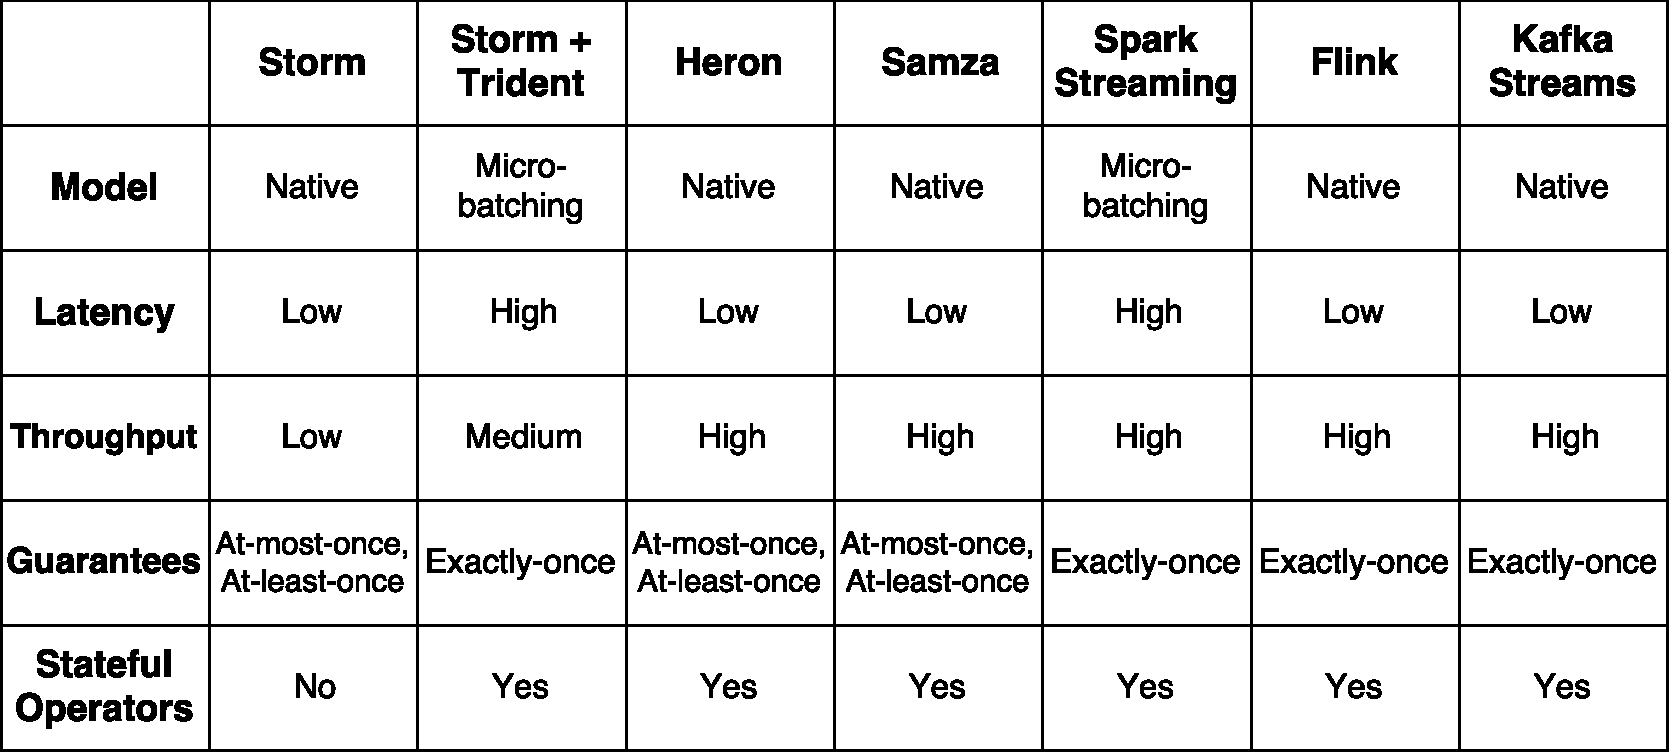
\includegraphics[width=1\textwidth]{images/streaming_engines.pdf}
 \caption{Streaming engines overview.}
\label{fig:streaming_engines_overview}
\end{figure}



An overview of the main features of the streaming frameworks discussed in the previous sections can be found in Figure \ref{fig:streaming_engines_overview}. We decided to evaluate Apache Spark Streaming, Flink and Kafka Streams. 
Apache Spark Streaming and Flink can be both good candidates because of their performances \cite{streamprocessingcomparison, yahoobenchmarkingonline, zalandobenchmarkingonline} and their maturity. They are also very flexible since they can be used as a single engine for both streaming and batch processing. Hence, they could be used as a single processing engine in the Lambda architecture. We chose also to test Kafka Streams because this system can be a good candidate for light-weight stream processing and we did not find any available benchmark of this system. 
%The result of the evaluation is available in Chapter 6. According to the results we obtained, Apache Flink is the streaming framework that better fits our uses cases. Thus, we decided to adopt Flink in our Cowbird architecture.

\section{Benchmarking Streaming Engines}
In this section we will portray the streaming engines benchmark framework we designed. We will report the results of the tests we performed on Apache Spark, Flink and Kafka Streams.
\subsection{The Benchmarking Framework}
\cite{yahoobenchmarkingonline, zalandobenchmarkingonline} designed a streaming engines benchmark that resembles their application scenario. Similar to what they have done, we designed a framework for evaluating streaming engines that recall our use cases. This approach can help us understanding which streaming framework is the most suitable for Cowbird. We tested Apache Spark Streaming (version 2.1.0), Apache Flink (version 1.2.0) and Kafka streams (Kafka version 0.10.2.0)

 \begin{figure}[h!]
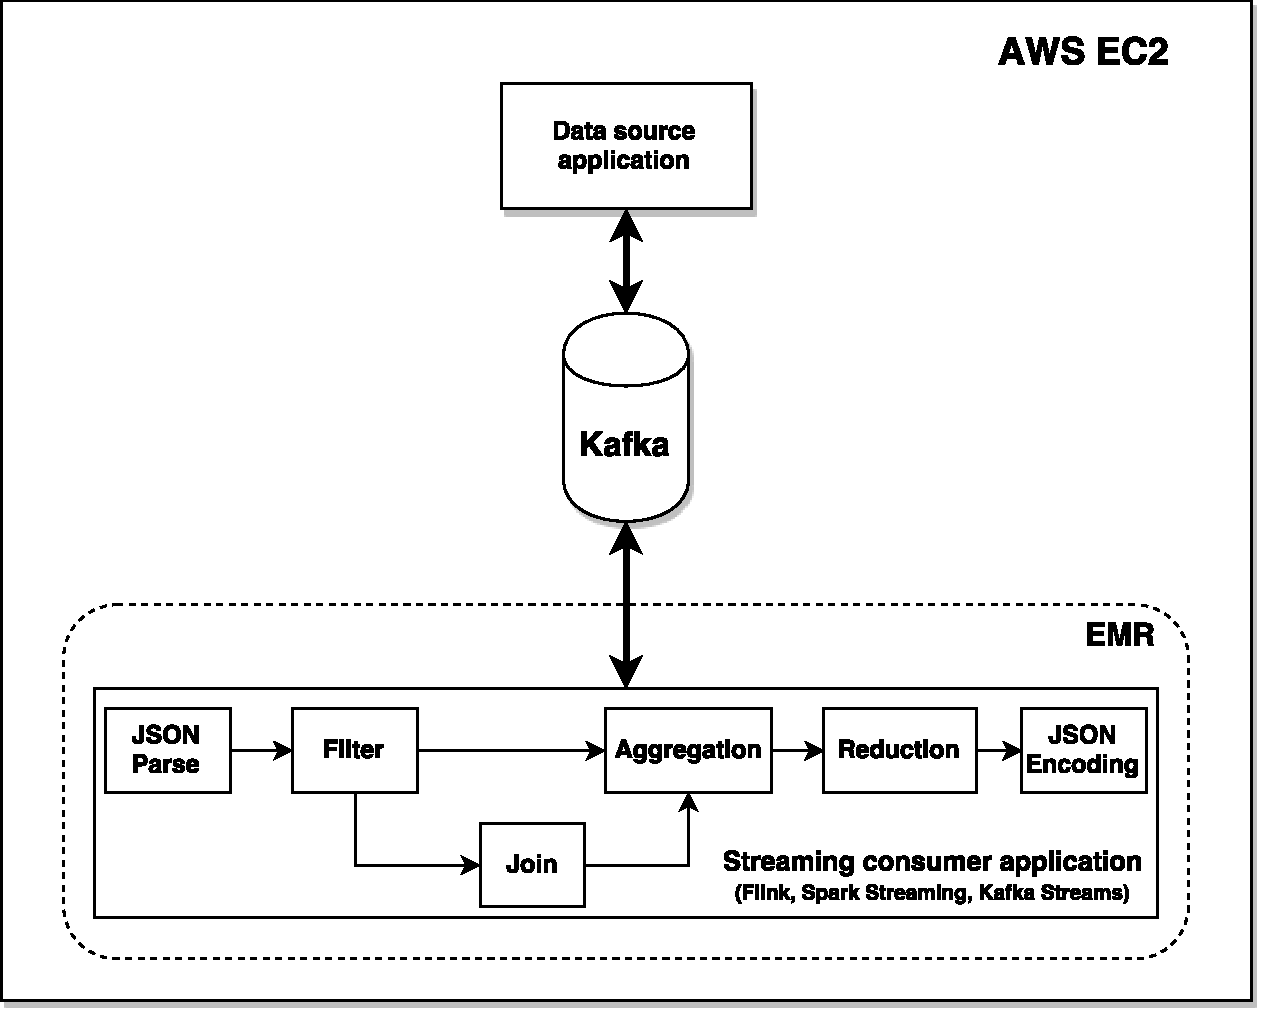
\includegraphics[width=1\textwidth]{images/benchmark.pdf}
 \caption{The streaming engines benchmark architecture.}
\label{fig:benchmark_architecture}
\end{figure}

Our benchmark framework contains (see Figure \ref{fig:benchmark_architecture}):
\begin{itemize}
\item A data source application that generates contents for a Kafka topic; each message generated contains an id that identifies a source, a double value, a reduction operation (i.e., MEAN, SUM, MAX and MIN), and the number of values required for applying the reduction operation (e.g., 1000 values coming from a source with a certain id). The data source application generates a certain number of events for a certain source and sends those to the Kafka broker. 
% batch??
The app can be tuned with some parameters provided by the user (e.g., number of sources, number of messages each source generates, the reduction operation to be performed on the data). 

%In Cowbird, instead, sensors data are generated This approach, indeed, can favorite the \emph{throughput}
%The SWAN framework processes sensors data values over a history time window while our benchmarking application process a certain number of values generated by a source. Hence, our benchmarking application can score a higher throughput since generated messages are sent in batch.

\item A streaming consumer application that runs on the streaming engine and applies the reduction operations. The application emits on Kafka the result for a certain source along with the time spent to compute the reduction operation. The time spent for computation is calculated as the difference between the time at the reduction evaluation and the timestamp of the first message received by Kafka from a certain source.
\end{itemize}

A consumer application has been designed for each of the three systems that have been tested. The consuming applications keep an \emph{incremental state} for each stream marked with a certain identifier. The incremental state stores only the partial result of the data that have been ingested so far into the system; this approach avoids to store all the records of data generated. The incremental state is calculated according to the reduction operator indicated for that stream. For example, in order to calculate the MEAN, the state will store the sum of the data values and the number of records that have flowed into the streaming engine. All the messages exhanged through the Kafka broker are in JSON format. The implementation of such benchmark framework can be found at \cite{streamingbenchmarkonline}

\subsection{Setup}
The evaluation has been done in a relatively simple setup on Amazon Web Services (AWS) \cite{amazonwebservicesonline}. The streaming engines are executed through EMR \cite{amazonemronline} on top of a small cluster composed of one master and two workers (m3.xlarge 4 vCPU, 15 GiB memory, 80 SSD GB storage each).
% The Kafka Streams application have been executed, instead, directly on three m3.xlarge instances using Amazon EC2 \cite{amazonec2online}.

Apache Kafka is executed in one broker instance along with Apache Zookeeper (m4.xlarge 4 vCPU, 16 GiB memory).

The streaming frameworks are executed using the default settings and we focused on writing correct, easy to understand programs without optimizing each streaming implementation to its full potential.

\subsection{Results}
We stressed all the three systems with different loads of messages containing double values. We use double values since many sensors produces measurements in such data format. In all the tests we performed the input messages have been processed using the MEAN history reduction mode. The batch duration in the Spark streaming was set to 1 second. In our tests, we focused on measuring how the tested systems react in terms of latency in situations of high input load.

\paragraph{}
Figure \ref{fig:results_100k} and Figure \ref{fig:results_1m} show the latency for various numbers of input messages per second. The results we obtained for Spark Streaming framework and Flink is similar to what was achieved by \cite{yahoobenchmarkingonline, zalandobenchmarkingonline}.

 \begin{figure}[h!]
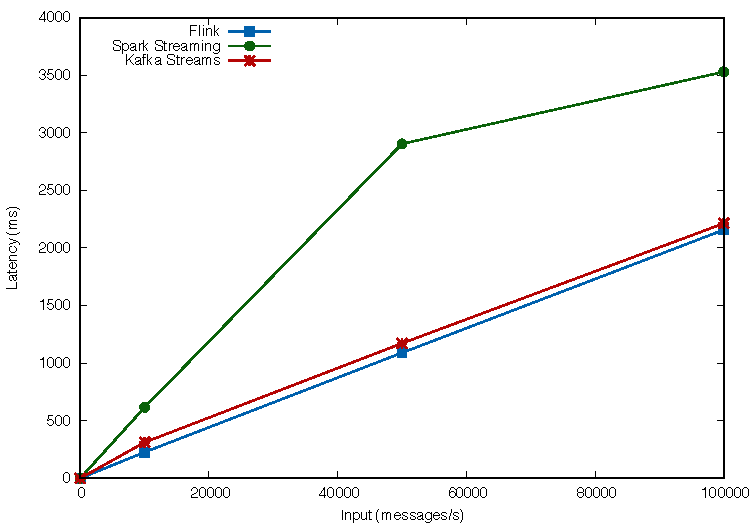
\includegraphics[width=1\textwidth]{images/engines_100k_cropped.pdf}
 \caption{Latencies evaluation up to 100K messages/s}
\label{fig:results_100k}
\end{figure}

 Kafka Streams performs very well and with a reasonable small input obtained performance similar to Apache Flink. Both Kafka Streams and Flink respond quite linearly. On the other hand, in Figure \ref{fig:results_100k} Spark Streaming behaves in a stepwise way; this could be a direct result from its micro-batching design. On drastically increasing the amount of input messages per second, all the three systems start suffering from the backpressure effect (the system is receiving data at a higher rate than it can process) also because of the limited setup configuration.
 
 \begin{figure}[h!]
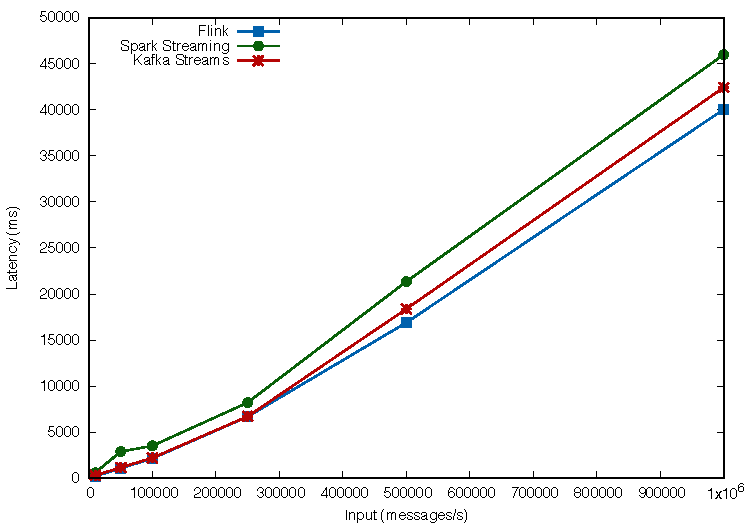
\includegraphics[width=1\textwidth]{images/engines_1m_cropped.pdf}
 \caption{Latencies evaluation up to 1M messages/s}
\label{fig:results_1m}
\end{figure}

 \begin{figure}[h!]
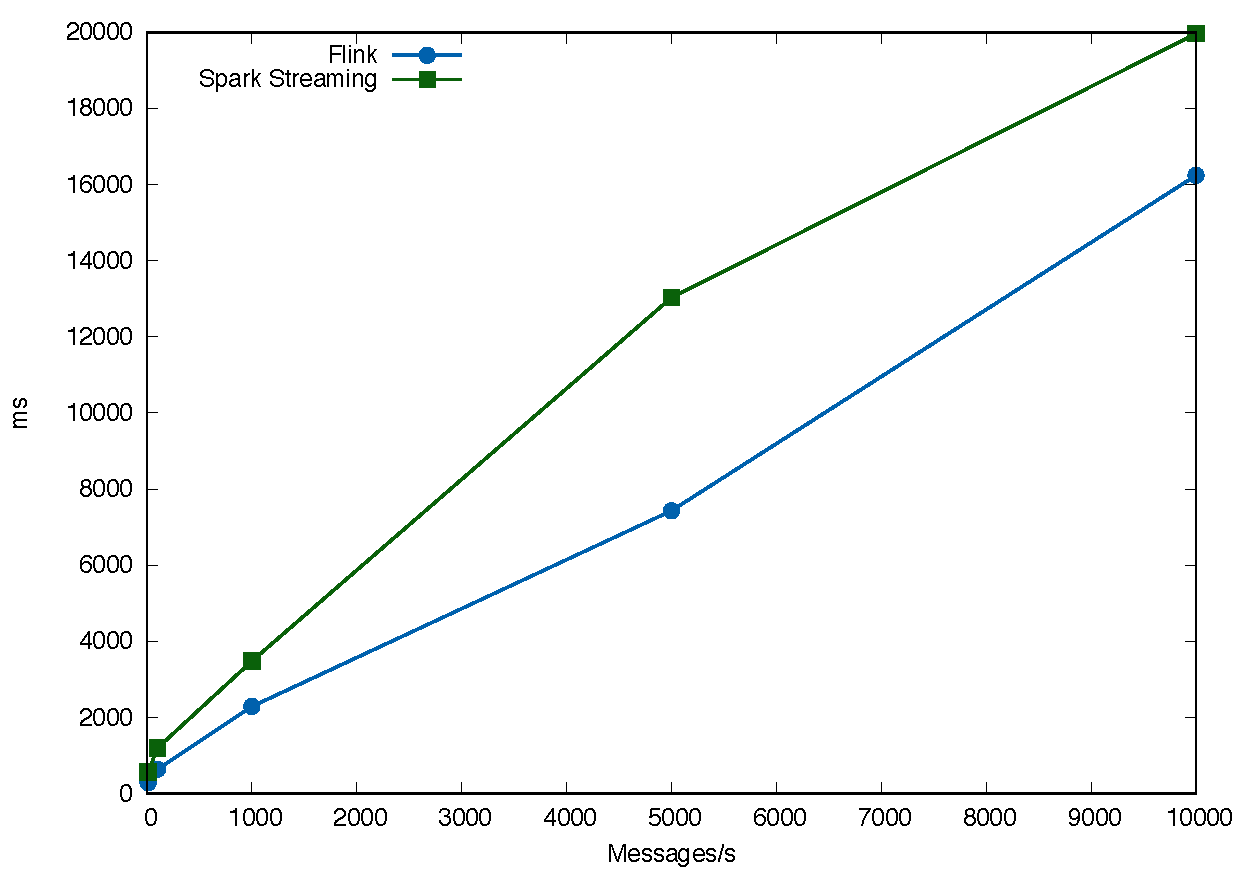
\includegraphics[width=1\textwidth]{images/join_cropped.pdf}
 \caption{Two streams JOIN-REDUCTION evaluation}
\label{fig:results_join}
\end{figure}


Figure \ref{fig:results_join} shows the evaluation result for join operations in Spark Streaming and Flink. In particular, the incoming streams of data (we set a window size of 1 second in Flink) are continuously joined with a set of 500MB pre-generated messages. The resulting streams of messages are then processed as usual. We notice that Flink has lower latency compared to Spark Streaming. We did not evaluate the join operation in Kafka Streams because such operator is not available for streams of data but only for tables.
\paragraph{}
The benchmark uses a naive setup and for this reason it can only give a sneak peek of the actual performance capabilities of the analyzed systems. Some of the achieved results are unacceptable or highly impractical for a real-time streaming application. However, this benchmark, even though executed on a relatively small scale, helped us understanding how the tested streaming engines can behave. Furthermore, in order to have a more detailed portrait of the tested engines fault tolerance and resources utilization should be evaluated as well. 
\paragraph{}
According to the results we obtained, Apache Flink is the streaming framework that better fits our uses cases. Nonetheless, it is important to outline that our naive benchmarking application is much less complex than the Cowbird framework. Furthermore, Cowbird evaluates sensors data records over a history time window while our benchmarking application processes a certain number of data values generated by a certain source without considering any windowing parameter.

%. Hence, our benchmarking application can score a higher throughput since generated messages are sent in batch.

%In Cowbird, instead, sensors data are generated This approach, indeed, can favorite the \emph{throughput}
%
